\documentclass[answers, 11pt]{exam}

\usepackage[spanish]{babel}
\usepackage[shortlabels]{enumitem}
\usepackage[T1]{fontenc}
\usepackage{amsmath}
\usepackage{graphicx}
\usepackage[cache=false,outputdir=./build]{minted}
\usepackage{lmodern}
\usepackage{wrapfig}
\usepackage{xcolor, color}
\definecolor{LightGray}{gray}{0.9}

\newcommand{\materia}{Analisis de Algoritmos 2024-1}
\newcommand{\tarea}{Tarea 09: Prim, Kruskal y Dijkstra}
\newcommand{\fecha}{\today}
\newcommand{\profesor}{Profesor(a): María de Luz Gasca Soto}
\newcommand{\ayudantes}{
  Rodrigo Fernando Velázquez Cruz \\
  Teresa Becerril Torres
}
\newcommand{\alumnos}{
  Alvaro Ramírez López \textbf{N° cuenta:} 316276355
}

\decimalpoint{}
\graphicspath{{img}}
% \colorsolutionboxes
\shadedsolutions

% \definecolor{SolutionBoxColor}{rgb}{0,128,255}
% \definecolor{SolutionColor}{rgb}{0,204,255}
\definecolor{SolutionColor}{rgb}{0,128,255}

\renewcommand{\familydefault}{\sfdefault}

\extrawidth{1.56cm}
\extraheadheight[1.5in]{-0.25in}
\extrafootheight[-0.175in]{-0.375in}
\firstpageheader{
}{
  \begin{minipage}[c]{3.5cm}
    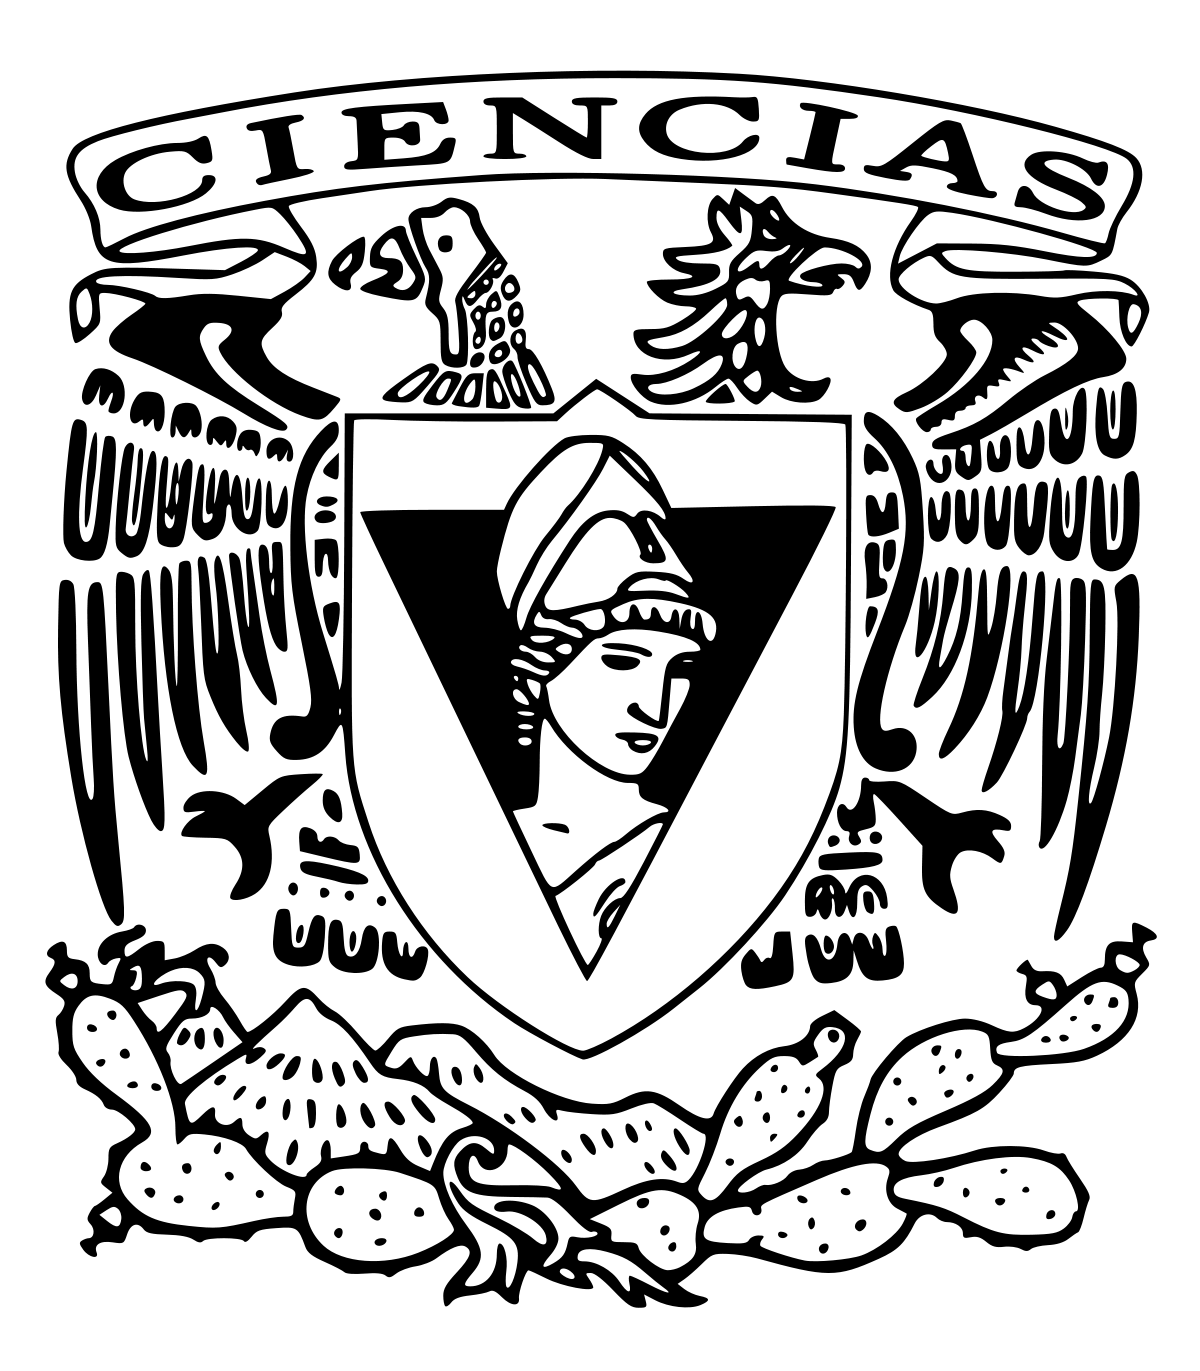
\includegraphics[width=3.5cm]{fc.png}
  \end{minipage}
  \begin{minipage}[c]{11.0cm}
    {\bfseries\huge\materia{} \\[2mm]
      \LARGE \tarea{} \\
      \large Profesor:} \profesor{} \\
    \hspace{0.1cm}
    {\bfseries\large Ayudantes:}
    \begin{minipage}[t]{8.5cm}
      \ayudantes{}\vspace{0.1cm}
    \end{minipage}\hfill\break{}
    {\bfseries\large Alumno:}
    \begin{minipage}[t]{8.5cm}
      \alumnos{}\\
    \end{minipage}\hfill\break{}
  \end{minipage}
  \begin{minipage}[c]{3.25cm}
    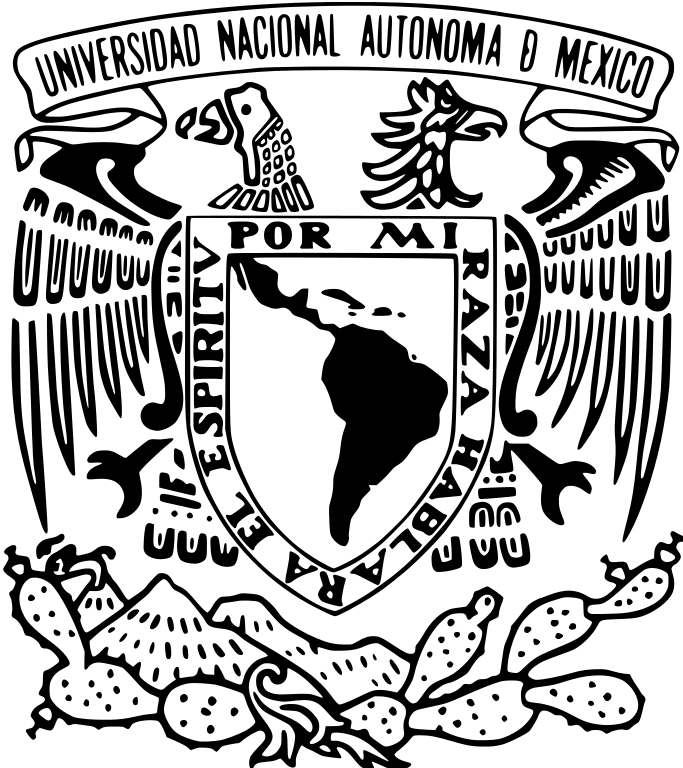
\includegraphics[width=3.25cm]{unam.png}
  \end{minipage}
}{}
\runningheader{\materia}{\tarea}{\fecha}
\runningheadrule{}
\footer{}{Página \thepage\ de \numpages}{}
\footrule{}
\renewcommand{\solutiontitle}{\noindent\textbf{Solución:}\par\noindent}



\begin{document}
\begin{questions}
  \question{Proporcionar una gráfica conexa $G = (V,A)$ con al menos 19 vértices
  y al menos 43 aristas con pesos positivos en el intervalo $[1,9] \subset Z$;
  deberá haber al menos cuatro aristas de cada costo $c$, $c\in[1,9]\subset Z$.
  Aplicar los siguientes algoritmos a la gráfica dada G, ilustrando cómo
  van transformandose las estructuras y mostrando al final los valores de
  las etiquetas para cada vértice.
  \begin{enumerate}[a)]
    \item Prim usando Heaps Binarios.
    \item Kruskal usando Conjuntos Ajenos con union por tamaño.
    \item Dijkstra usando Colas Binomiales.
    Modificar la gráfica $G = (V, A)$ dada: seleccionar un vértice como
    fuente, $s$, y dar dirección a las aristas para aplicar Dijsktra.
  \end{enumerate}
  }

  \question{Sea a una arista de peso mínimo de una gráfica $G=(V,A)$ con pesos
  en las aristas.
  \begin{enumerate}[a)]
    \item Modificar tanto el Algoritmo Prim como el Kruskal para que
    la arista a siempre aparezca en el árbol generador de peso mínimo.
    \item Calcular el desempeño computacional de los algoritmos propuestos,
    indicando las estructuras de datos usadas para lograr tal desempeño.
  \end{enumerate}}

  \begin{solution}
    Para lograr que una arista específica, denotada como 'a', siempre aparezca 
    en el árbol generador de peso mínimo, se pueden realizar modificaciones en 
    los algoritmos de Prim y Kruskal. A continuación, se presentan las modificaciones 
    para ambos algoritmos:

\textbf{Modificación del Algoritmo de Prim:}

\begin{enumerate}
  \item \textbf{Inicialización:}
  Inicializa el árbol generador mínimo con la arista 'a'.

  \item \textbf{Selección de la Arista:}
  En cada paso, selecciona la arista de peso mínimo que conecta un vértice en el 
  árbol actual con un vértice fuera del árbol, garantizando que la arista 'a' 
  siempre sea seleccionada si es posible.

  \item \textbf{Actualización de Conjuntos:}
  Actualiza los conjuntos de vértices que forman parte del árbol y los que están 
  fuera del árbol.

  \item \textbf{Repetición:}
  Repite el proceso hasta que todos los vértices estén en el árbol generador mínimo.
\end{enumerate}

\textbf{Modificación del Algoritmo de Kruskal:}

\begin{enumerate}
  \item \textbf{Orden de las Aristas:}
  Antes de comenzar el algoritmo, asegúrate de que la arista 'a' esté incluida 
  en la lista de aristas y se ordene primero.

  \item \textbf{Unión de Conjuntos:}
  Durante la ejecución del algoritmo, al unir dos conjuntos de vértices, verifica 
  que la arista 'a' esté incluida en el árbol generador mínimo.

  \item \textbf{Repetición:}
  Continúa con el proceso hasta que todos los vértices estén en un solo conjunto.

\end{enumerate}

\textbf{Desempeño Computacional:}

El desempeño computacional de ambos algoritmos dependerá en gran medida de las 
estructuras de datos utilizadas. Aquí hay algunas consideraciones generales:

\textbf{Algoritmo de Prim modificado:}

\begin{itemize}
  \item \textbf{Estructura de Datos para Mantener las Aristas:}
  Puedes usar una cola de prioridad (heap binario o Fibonacci) para mantener las 
  aristas ordenadas por peso.
  
  \item \textbf{Estructura de Datos para Mantener Conjuntos de Vértices:}
  Puedes usar una estructura de conjunto disjunto (Union-Find) para realizar 
  operaciones de unión y encontrar eficientemente.
\end{itemize}

\textbf{Algoritmo de Kruskal modificado:}

\textbf{Estructura de Datos para Mantener las Aristas:}
  Al igual que en Prim, una cola de prioridad es útil para mantener las aristas 
  ordenadas por peso.

\textbf{Estructura de Datos para Mantener Conjuntos de Vértices:}
  También puedes usar una estructura de conjunto disjunto (Union-Find) para 
  realizar las operaciones de unión y encontrar de manera eficiente.

En términos de complejidad temporal, tanto Prim como Kruskal tendrán una complejidad 
de $O(E \log V)$, donde $E$ es el número de aristas y $V$ es el número de vértices. 
Las operaciones de conjuntos disjuntos son cruciales para lograr eficiencia en ambos algoritmos.

Es importante señalar que la complejidad exacta dependerá de la implementación 
específica y de la elección de las estructuras de datos.
  \end{solution}
  
  \question{
    Proyecto $\Gamma$: Sea $D=(V,A,\delta)$ una gráfica disconexa con pesos sobre
las aristas, con $|V|=n$, $|A|=m$ y $\delta:A\to R+$.
\begin{enumerate}[a)]
  \item Diseñar un algoritmo que determine el bosque generador de peso mínimo para D, 
  el algoritmo debe tener complejidad $O(m \log m)$, en el peor de los casos.
  El algoritmo debe ser capaz de mostrar los árboles obtenidos y los correspondientes pesos.

  \item Indicar las Estructuras de Datos con las que se alcanza el tiempo pedido 
  y justificar formalmente el desempeño computacional del algoritmo propuesto.
  
  \item Proporcionar una gráfica D con al menos 27 vértices, al menos 39 aristas 
  con pesos positivos y al menos cuatro componentes conexas.
  Aplicar detalladamente el algoritmo propuesto en el Ejercicio 3 a la gráfica 
  disconexa D creada.
\end{enumerate}}

\begin{solution}
  Aqui esta la solucion del problema 3.
\end{solution}

  \question{\textbf{Opcional.} Sea $G=(V,A)$ una gráfica conexa con pesos positivos
  sobre las aristas. Supongamos que el costo de un árbol generador se define como 
  el producto de los costos en las aristas
  \begin{enumerate}[a)]
    \item Diseñar un algoritmo que determine el árbol generador de peso
    máximo, usando tal regla.
    
    \item Calcular el desempeño computacional del algoritmo propuesto, indicando 
    las estructuras de datos usadas para lograr tal desempeño.
  \end{enumerate}}

  \begin{solution}
    \textbf{a)Diseñar un algoritmo que determine el árbol generador de peso
    máximo, usando tal regla.}

    Para resolver este problema, puedes utilizar el algoritmo de Kruskal modificado 
    para maximizar el peso del árbol generador. Aquí te doy una descripción del 
    algoritmo y luego abordo la cuestión del desempeño computacional y las 
    estructuras de datos utilizadas.

    Algoritmo para encontrar el árbol generador de peso máximo:
    
    \begin{enumerate}[1.]
      \item \textbf{Ordenar las aristas:} Ordena todas las aristas en orden no decreciente de peso.
      \item \textbf{Inicializar el árbol generador:} Inicializa un árbol generador vacío.
      \item \textbf{Agregar aristas de mayor a menor:} Recorre las aristas ordenadas de mayor a menor 
      peso y agrega cada arista al árbol generador si no forma un ciclo con las aristas 
      ya seleccionadas.
    \end{enumerate}

    Este enfoque modificado del algoritmo de Kruskal seleccionará aristas de mayor 
    peso en lugar de menor peso, asegurando así que el árbol generador 
    resultante tenga el peso máximo.

    \textbf{b) Calcular el desempeño computacional del algoritmo propuesto, indicando 
    las estructuras de datos usadas para lograr tal desempeño.}

    \textbf{Ordenar las aristas:} Este paso requiere tiempo $(O(E \log E))$, 
    donde $(E)$ es el número de aristas.
  
    \textbf{Estructuras de datos:} Para mantener el seguimiento de los conjuntos 
    disjuntos y verificar si agregar una arista forma un ciclo, puedes utilizar 
    una estructura de datos eficiente como una estructura de conjuntos disjuntos 
    (Disjoint Set Union, DSU). La operación de unión en DSU puede realizarse en 
    $(O(\alpha(V)))$ en promedio, donde $(\alpha(V))$ es la inversa de la función 
    de Ackermann, y $(V)$ es el número de vértices.

    \textbf{Recorrer las aristas ordenadas:} Este paso tiene un tiempo de ejecución 
    de $(O(E))$, ya que se recorren todas las aristas una vez.

    Por lo tanto, el tiempo total de ejecución es dominado por el costo de ordenar 
    las aristas, lo que resulta en $(O(E \log E))$ en el peor de los casos.

    El espacio adicional requerido para mantener la estructura de conjuntos disjuntos 
    y otras variables auxiliares es $(O(V + E))$.

    En resumen, el desempeño computacional del algoritmo propuesto es 
    $(O(E \log E))$, y las estructuras de datos utilizadas son principalmente 
    la estructura de conjuntos disjuntos y un arreglo para mantener las aristas ordenadas.
  \end{solution}
  
\end{questions}
\end{document}